\documentclass[a4paper,twoside]{article}
\usepackage[T1]{fontenc}
\usepackage[bahasa]{babel}
\usepackage{graphicx}
\usepackage{graphics}
\usepackage{float}
\usepackage[cm]{fullpage}
\pagestyle{myheadings}
\usepackage{etoolbox}
\usepackage{setspace} 
\usepackage{lipsum} 
\usepackage{hyperref}
\graphicspath{ {./images/} }
\setlength{\headsep}{30pt}
\usepackage[inner=2cm,outer=2.5cm,top=2.5cm,bottom=2cm]{geometry} %margin
% \pagestyle{empty}

\makeatletter
\renewcommand{\@maketitle} {\begin{center} {\LARGE \textbf{ \textsc{\@title}} \par} \bigskip {\large \textbf{\textsc{\@author}} }\end{center} }
\renewcommand{\thispagestyle}[1]{}
\markright{\textbf{\textsc{AIF234001 \textemdash Rencana Kerja Tugas Akhir \textemdash Sem. Ganjil 2023/2024}}}

\newcommand{\HRule}{\rule{\linewidth}{0.4mm}}
\renewcommand{\baselinestretch}{1}
\setlength{\parindent}{0 pt}
\setlength{\parskip}{6 pt}

\onehalfspacing
 
\begin{document}

\title{\@judultopik}
\author{\nama \textendash \@npm} 

%tulis nama dan NPM anda di sini:
\newcommand{\nama}{Nathanael Adi Trianto}
\newcommand{\@npm}{6181901041}
\newcommand{\@judultopik}{Pembuatan Ulang Aplikasi Rugby Indonesia dengan Ionic 7 dan Capacitor} % Judul/topik anda
\newcommand{\jumpemb}{1} % Jumlah pembimbing, 1 atau 2
\newcommand{\tanggal}{22/09/2023}

% Dokumen hasil template ini harus dicetak bolak-balik !!!!

\maketitle

\pagenumbering{arabic}

\section{Deskripsi}
\textit{Rugby} adalah olahraga tim yang berasal dari abad ke-19 sebagai variasi sepak bola. Dalam \textit{rugby}, tujuannya adalah meletakkan bola di belakang garis coba lawan. Ini dimainkan dengan tangan dan tendangan, tetapi bola hanya boleh dilempar atau diserahkan ke belakang saat dibawa tangan. \textit{Rugby} berbeda dari sepak~bola~Amerika.

Olahraga ini bisa dimainkan oleh siapa saja yang memiliki sepatu sepak bola, perlengkapan olahraga, dan pelindung mulut. Latihan meliputi teknik, koordinasi, dan kendali bola. \textit{Rugby} adalah olahraga kontak penuh yang memerlukan kekuatan, ketangguhan, kecerdikan, dan kendali tubuh.

Permainan ini dimainkan secara \textit{scrum}. \textit{Scrum} adalah bagian penting dalam permainan, dimulai setelah pelanggaran aturan. Pemain depan bergabung untuk merebut bola dalam \textit{scrum}. Ada juga \textit{line-out} yang digunakan ketika bola keluar lapangan.


% Rugby adalah salah satu olahraga bola yang dimainkan oleh dua tim. Berdasarkan jumlah pemainnya, olahraga rugby terbagi menjadi 3 jenis utama, yaitu:

% \begin{itemize}
%     \item Rugby union: setiap tim terdiri dari 15 pemain.
%     \item Liga rugby: setiap tim terdiri dari 13 pemain.
%     \item Rugby sevens: setiap terdiri dari 7 pemain.
% \end{itemize}

% Masing-masing tim diharuskan untuk mencetak poin dengan menendang, melempar, membawa dan mendaratkan bola melewati gawang atau garis belakang tim lawan.

% Bola yang digunakan pada olahraga rugby memiliki ciri khas, yaitu berbentuk lonjong dan mengerucut pada bagian ujungnya. Dengan bentuknya ini, bola rugby jadi lebih mudah dipegang dan dibawa oleh para pemain selama pertandingan berlangsung.

Sejarah permainan \textit{rugby} dimulai pada tahun 1886, terjadi perdebatan mengenai sebuah percobaan dalam permainan \textit{rugby}, yang kemudian memunculkan pembentukan Dewan \textit{Rugby} Sepak Bola Internasional oleh serikat \textit{rugbi} dari Irlandia, Skotlandia, dan Wales. Mereka mengusulkan pembentukan dewan netral untuk menetapkan dan mengatur aturan \textit{rugby}. Rugby Football Union, yang merupakan serikat pertama dan tertua, kemudian bergabung dengan IRFB pada tahun 1890 dan memiliki setengah dari 12 suara, sementara serikat pendiri masing-masing memiliki dua suara.

% Susunan dewan dan alokasi kursinya berubah seiring dengan popularitas permainan yang tumbuh. Selandia Baru, Afrika Selatan, dan Australia bergabung pada tahun 1949, tetapi baru 29 tahun kemudian Prancis menjadi anggota kedelapan IRFB. Pengenalan Piala Dunia Rugbi pada tahun 1987 memicu penyebaran permainan ini ke seluruh dunia, dan anggota IRFB bertambah pesat menjelang akhir abad ini.

Pertumbuhan ini berlanjut hingga saat ini, dengan Republik Demokratik Kongo, Mesir, dan Suriah menjadi anggota terbaru World Rugby pada November 2022, sehingga total anggota mencapai 132 serikat.

% Organisasi pengatur ini mengawasi perkembangan profesionalisme pada Agustus 1995 dan tiga tahun kemudian berganti nama menjadi Dewan Rugbi Internasional. Pada Oktober 2009, \textit{rugby} tujuh pemain kembali masuk dalam program Olimpiade, dan pada November 2014, berganti nama menjadi World Rugby sebagai bagian dari \textit{rebranding} besar.

Persatuan Rugby Union Indonesia (PRUI) adalah organisasi yang bertanggung jawab atas pengelolaan dan pengembangan Rugby Union di Indonesia. PRUI adalah asosiasi olahraga yang sepenuhnya diakui di Indonesia dan telah menjadi anggota penuh Asia Rugby dan World Rugby. PRUI memiliki tim nasional putra dan putri yang berkompetisi dalam acara tunggal. Rugby Union di Indonesia adalah olahraga yang sedang berkembang dan telah mengalami fluktuasi dalam kesuksesannya. Didik Mukrianto saat ini menjabat sebagai Ketua Umum PRUI untuk masa bakti 2021-2025 setelah terpilih dalam Musyawarah Olahraga Nasional (Musornas) ketiga

% dari kota Rugby, Inggris pada tahun 1823. Permainan tersebut dicetuskan oleh seorang pemuda bernama William Webb Ellis ketika bermain sepak bola dengan teman-temannya, William mengambil bola dan berlari menuju gawang tim lawan untuk mencetak skor. Seiring berjalannya waktu, rugby terus berkembang dan membentuk federasinya yang pertama, yaitu Rugby Football Union, pada tahun 1871. Keberhasilannya semakin mengukuhkan statusnya ketika rugby pertama kali dipertandingkan secara resmi dalam ajang turnamen olahraga internasional yaitu Olimpiade, pada tahun 1900. Meskipun sempat absen dari Olimpiade pada tahun 1924, rugby kembali sebagai cabang olahraga resmi dalam turnamen Olimpiade tahun 2016 dan tetap relevan hingga saat ini.

Ionic Framework adalah \textit{toolkit UI open-source} untuk membangun aplikasi modern, \textit{cross-platform} yang berkualitas tinggi dari satu kode sumber dengan JavaScript dan web. Ionic menyediakan alat dan layanan untuk mengembangkan aplikasi\textit{ hybrid mobile, desktop}, dan \textit{progressive web} berdasarkan teknologi dan praktik pengembangan web modern, menggunakan teknologi web seperti CSS, HTML5, dan Sass. Ionic 7 adalah versi \textit{stable release} terbaru dari Ionic, yang memperkenalkan cara kerja yang lebih efisien dengan kontrol formulir seperti \textit{Toggle} atau \textit{Input}. Komponen \textit{Item} dan Label tidak lagi diperlukan, dan setiap kontrol formulir menangani konten label secara langsung. Selain itu, fitur tertentu seperti teks bantuan atau mode pengisian \textit{input} telah dipindahkan dari ion-item ke kontrol formulir yang sesuai seperti ion-input, ion-textarea, dan ion-select. Perubahan ini mengurangi \textit{boilerplate} kode dengan menghilangkan persyaratan ion-item dan ion-label. Komponen Ionic Framework secara otomatis menyesuaikan tampilan dan nuansa mereka dengan platform di mana mereka berjalan, memungkinkan gestur dan perilaku native yang sama dengan yang biasa digunakan pengguna. Ionic memiliki lebih dari 100 komponen \textit{UI} yang telah dirancang sebelumnya, tipografi, dan tema dasar yang menyesuaikan dengan setiap platform. Ini dioptimalkan untuk \textit{mobile} dengan animasi yang diakselerasi oleh \textit{hardware}, \textit{lazy loading}, dan \textit{scrolling 60FPS}. Ionic CLI digunakan untuk membuat, membangun, dan menguji aplikasi serta memanfaatkan\textit{ Live Reload, deployment}, dan dokumen~yang~sangat~baik.

Capacitor adalah \textit{runtime native cross-platform} yang memudahkan pembuatan aplikasi \textit{mobile} yang performanya tinggi dan berjalan secara \textit{native} di iOS, Android, dan platform lainnya menggunakan \textit{web tooling modern}. Capacitor merupakan evolusi selanjutnya dari aplikasi \textit{hybrid}, yang menciptakan aplikasi \textit{Web Native} dengan pendekatan \textit{native container} modern untuk tim yang ingin membangun aplikasi \textit{web-first} tanpa mengorbankan akses penuh ke \textit{SDK native} ketika dibutuhkan. Capacitor menyediakan kumpulan API yang konsisten dan berfokus pada web yang memungkinkan aplikasi tetap dekat dengan standar web sebanyak mungkin, sambil mengakses fitur perangkat \textit{native} yang kaya pada platform yang mendukungnya. Capacitor dapat menambahkan fungsionalitas \textit{native} dengan mudah menggunakan \textit{Plugin} API untuk Swift di iOS, Java di Android, dan JavaScript untuk web. Capacitor 3.0 memiliki peningkatan kinerja, pengalaman untuk mengembangkan yang lebih baik, dan keterlibatan komunitas yang lebih besar. Capacitor dapat diintegrasikan dengan mudah ke dalam proyek JavaScript modern yang ada atau proyek Capacitor yang~baru.

Sekitar tahun 2015, perusahaan PT DNArtworks Komunikasi Visual membuat aplikasi Rugby Indonesia yang memanfaatkan Apache Cordova. Aplikasi tersebut memiliki: 
\begin{itemize}
    \item Halaman \textit{Latest News} yang diambil dari \url{https://rugbyindonesia.or.id} dengan~memanfaatkan~protokol~RSS.
    \item Halaman \textit{Fixture \& Results} yang diambil dari \url{https://rugbyindonesia.or.id}.
    \item Halaman \textit{Teammate Photos} dengan fungsi:
    \begin{itemize}
        \item Pengguna dapat langsung mengambil foto dari aplikasi tersebut.
        \item Pengguna dapat langsung memberikan frame terhadap foto tersebut.
        \item Pengguna dapat langsung menggunggah foto tersebut ke dalam galeri publik.
    \end{itemize}
    \item Halaman \textit{Rugby Clubs} yang memiliki fungsi di mana pengguna dapat langsung mendaftar ke dalam klub rugbi yang berada di Indonesia.
    \item Fungsi \textit{Push Notifications}.
\end{itemize}

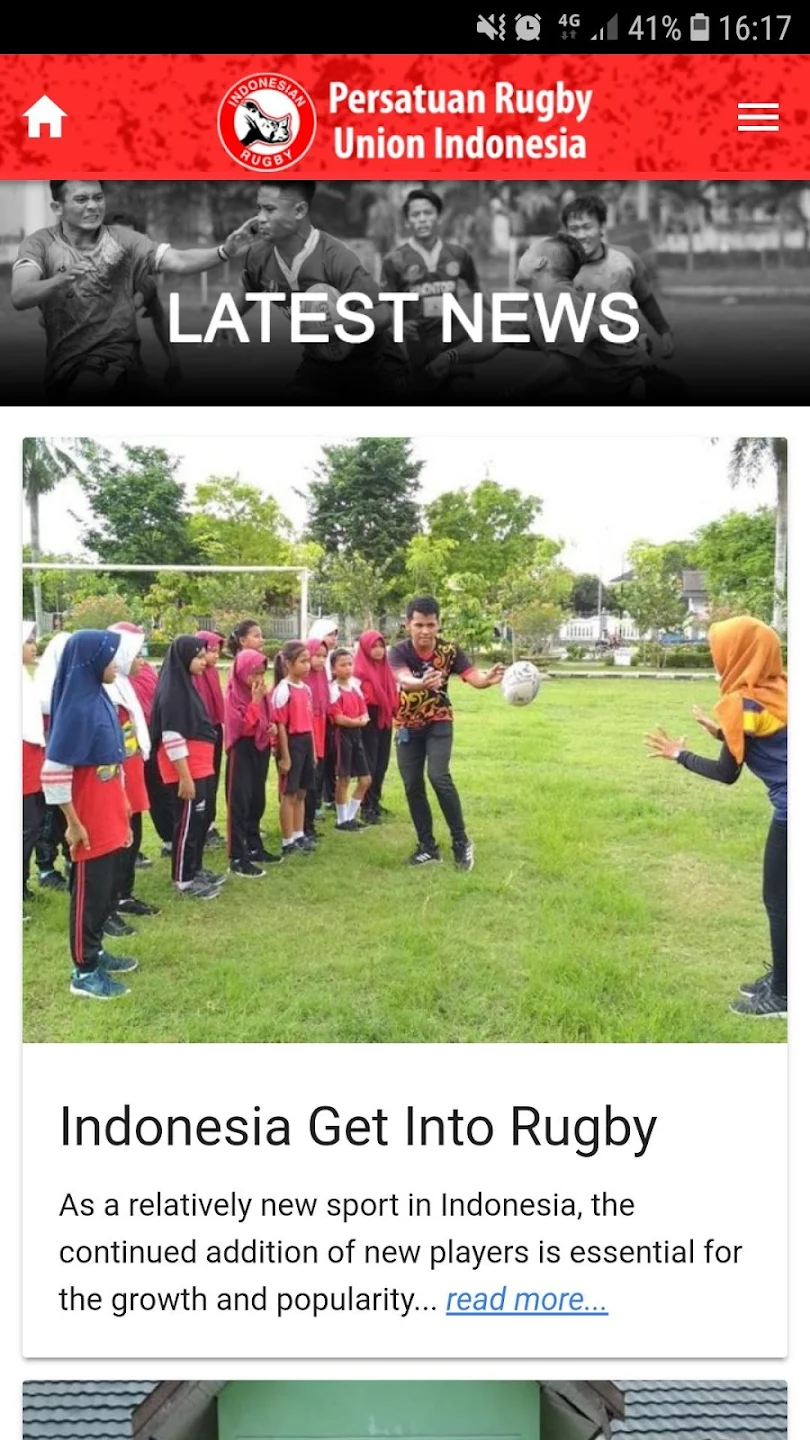
\includegraphics[scale=0.125]{latest_news.png} \hspace{0.5cm}
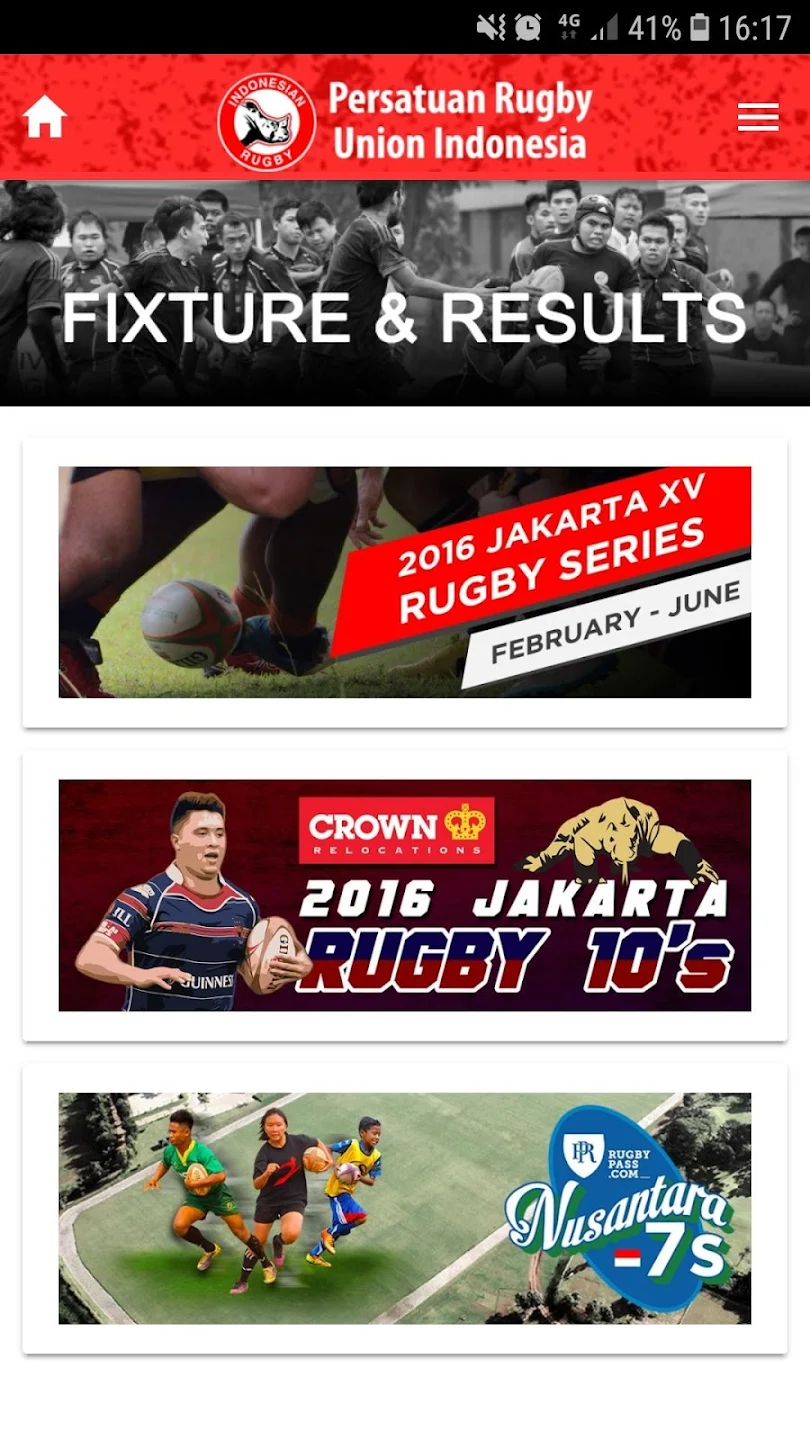
\includegraphics[scale=0.125]{fixture_results.png} \hspace{0.5cm}
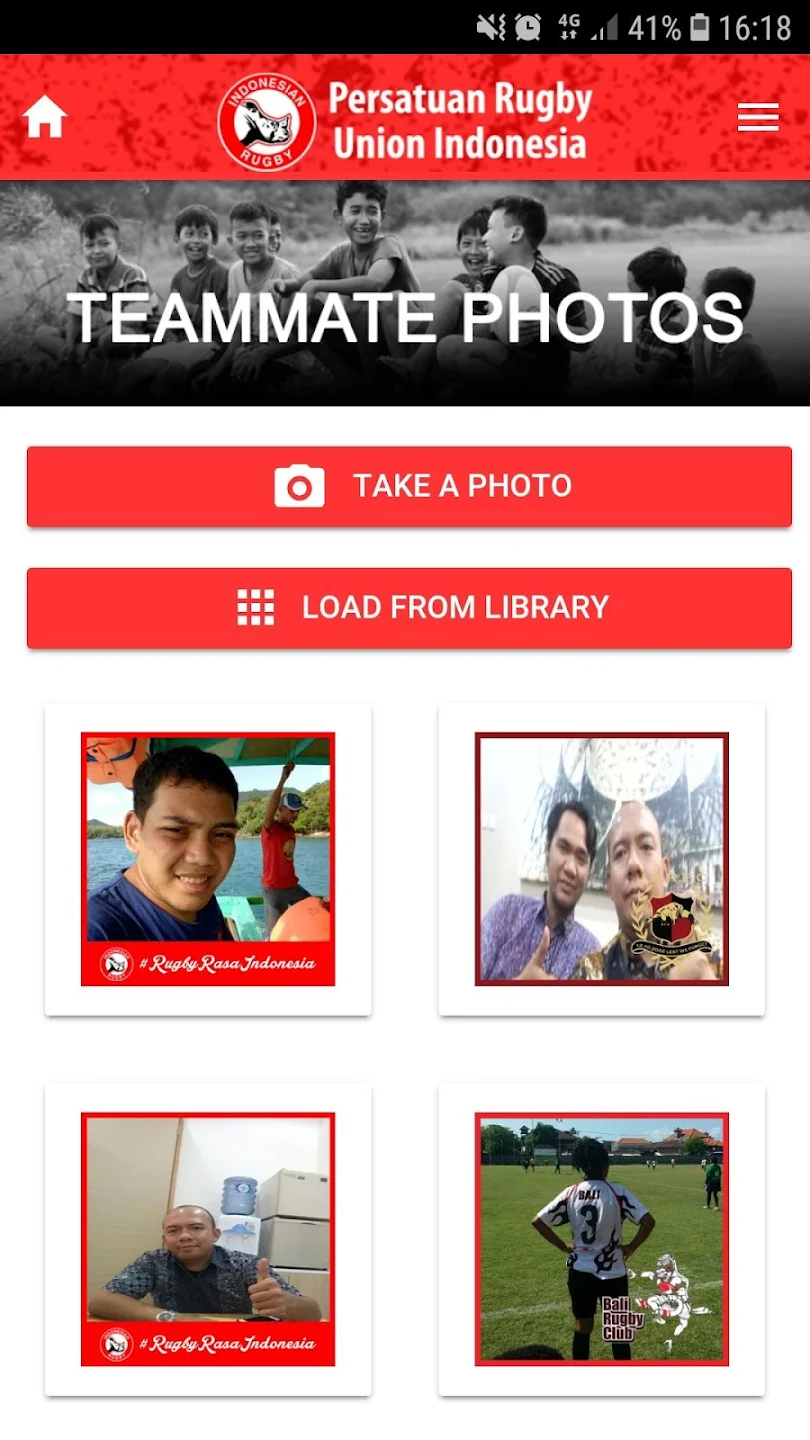
\includegraphics[scale=0.125]{teammate_photos.png} \hspace{0.5cm}
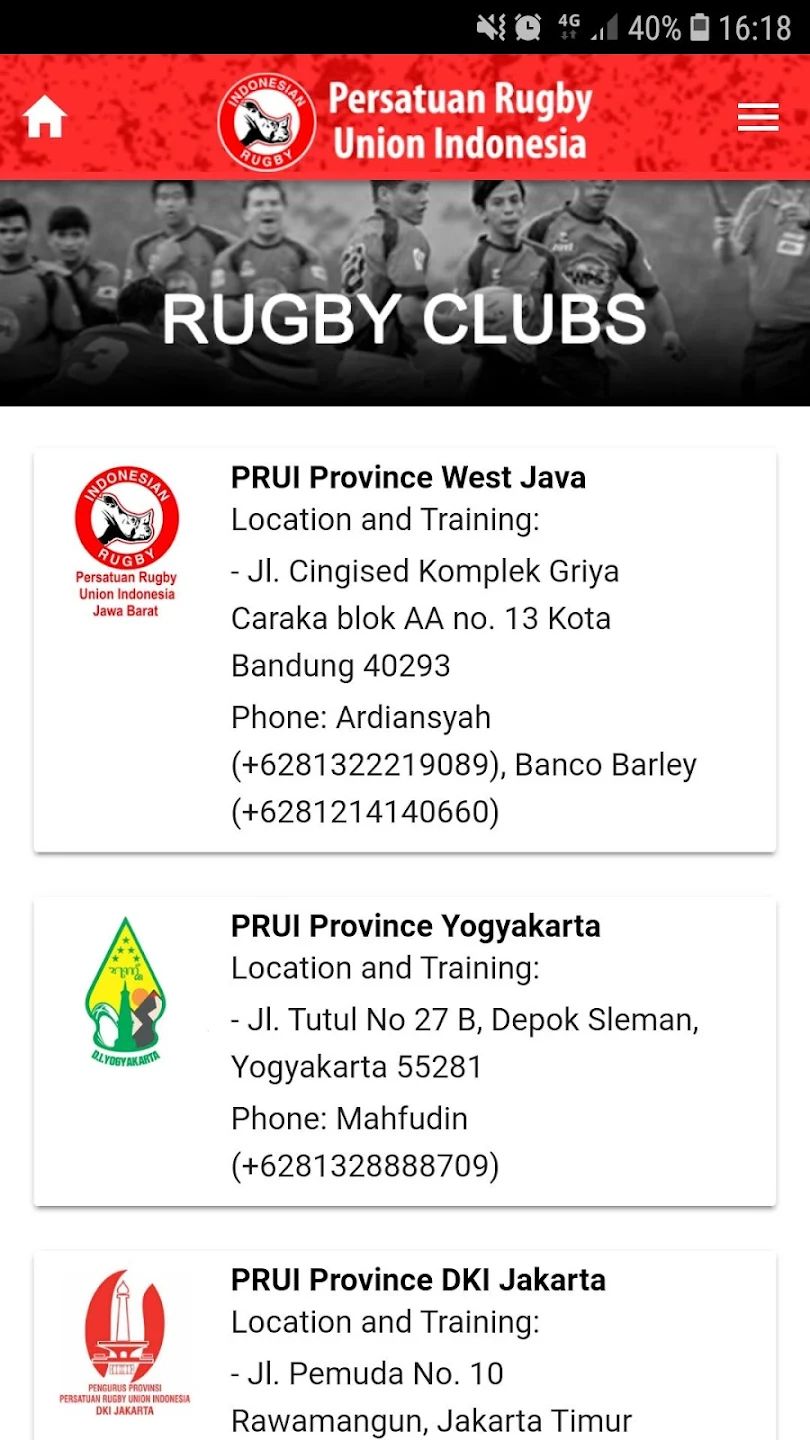
\includegraphics[scale=0.125]{rugby_clubs.png}

Pada saat ini, aplikasi tersebut masih tersedia di \href{https://play.google.com/}{Google Play Store}, namun aplikasi tersebut tidak dapat dipasang pada perangkat \textit{android} saat ini dikarenakan website \url{https://rugbyindonesia.or.id} sudah berubah dan juga framework yang digunakan sudah terlalu lama. Maka dari itu pada skripsi ini, akan dibuat ulang sebuah perangkat lunak Rugby Indonesia yang terbaru, sehingga perangkat lunak tersebut dapat \textit{compatible} dengan perangkat \textit{android} saat ini.

Perangkat lunak ini akan dibuat dengan memanfaatkan bantuan {\it framework} Ionic 7 dan Capacitor dengan:

\begin{itemize}
    \item Halaman \textit{Latest News}, di mana pengguna dapat melihat berita terbaru seputar Rugby Indonesia.
    \item Halaman \textit{Teammate Photos}.
\end{itemize}


\section{Rumusan Masalah}
Rumusan masalah yang akan dibahas pada skripsi ini adalah sebagai berikut:
\begin{itemize}
    \item Bagaimana cara mengembangkan perangkat lunak Rugby Indonesia dengan memanfaatkan \textit{framework} Ionic 7?
    \item Bagaimana cara menggunakan Capacitor pada pembangunan perangkat lunak Rugby Indonesia agar pengguna dapat mengunggah foto dengan mudah?
\end{itemize}

\section{Tujuan}
Tujuan yang ingin dicapai pada penulisan skripsi ini yaitu:
\begin{itemize}
    \item Dapat mengetahui bagaimana Ionic 7 memungkinkan pengembangan aplikasi Rugby Indonesia.
    \item Mengidentifikasi cara kerja dari Capacitor pada pembangunan perangkat lunak Rugby Indonesia.
\end{itemize}

\section{Deskripsi Perangkat Lunak}

Perangkat lunak akhir yang akan dibuat memiliki fitur minimal sebagai berikut:
\begin{itemize}
    \item Pengguna dapat melihat berita terbaru yang terdapat pada Rugby Indonesia.
    \item Pengguna dapat melihat foto yang diunggah oleh pengguna tersebut maupun pengunggah lain pada aplikasi Rugby Indonesia.
    \item Pengguna dapat megunduh foto yang terdapat pada aplikasi Rugby Indonesia.
    \item Pengguna dapat mengubah ataupun menghapus unggahan foto pengguna tersebut pada aplikasi Rugby Indonesia, namun tidak dapat melakukan hal tersebut pada foto yang diunggah oleh orang lain.
\end{itemize}

\section{Detail Pengerjaan Tugas Akhir}
Bagian-bagian pekerjaan skripsi ini adalah sebagai berikut :
\begin{enumerate}
    \item Mendalami ReactJS sebagai salah satu perpustakaan JavaScript.
    \item Menganalisis aplikasi Rugby Indonesia yang sudah dibuat dengan memanfaatkan Apache Cordova.
    \item Menganalisis fitur-fitur yang dibutuhkan untuk aplikasi Rugby Indonesia.
    \item Membuat aplikasi Rugby Indonesia yang sudah memanfaatkan \textit{framework} Ionic 7 dan juga Capacitor.
    \item Melakukan pengujian dan eksperimen.
    \item Menulis dokumen skripsi
\end{enumerate}

\section{Rencana Kerja}
Rincian capaian yang direncanakan di Tugas Akhir 1 adalah sebagai berikut:
\begin{enumerate}
    \item Mempelajarai, memahami, serta mendalami ReactJS sebagai salah satu perpustakaan JavaScript yang akan digunakan pada skripsi ini.
    \item Mempelajari, memahami, dan mendalami framework Ionic 7 serta Capacitor.
    \item Menganalisis kebutuhan fitur yang diperlukan untuk aplikasi Rugby Indonesia.
    \item Menulis dokumen tugas akhir.
\end{enumerate}

Sedangkan yang akan diselesaikan di Tugas Akhir 2 adalah sebagai berikut:
\begin{enumerate}
    \item Membuat aplikasi Rugby Indonesia yang sudah memanfaatkan framework Ionic 7 serta Capacitor.
    \item Melakukan pengujian dan juga eksperimen terhadap aplikasi yang akan dibuat.
    \item Menulis dokumen tugas akhir.
\end{enumerate}

\vspace{1cm}
\centering Bandung, \tanggal\\
\vspace{2cm} \nama \\ 
\vspace{1cm}

Menyetujui, \\
\ifdefstring{\jumpemb}{2}{
\vspace{1.5cm}
\begin{centering} Menyetujui,\\ \end{centering} \vspace{0.75cm}
\begin{minipage}[b]{0.45\linewidth}
% \centering Bandung, \makebox[0.5cm]{\hrulefill}/\makebox[0.5cm]{\hrulefill}/2013 \\
\vspace{2cm} Nama: \makebox[3cm]{\hrulefill}\\ Pembimbing Utama
\end{minipage} \hspace{0.5cm}
\begin{minipage}[b]{0.45\linewidth}
% \centering Bandung, \makebox[0.5cm]{\hrulefill}/\makebox[0.5cm]{\hrulefill}/2013\\
\vspace{2cm} Nama: \makebox[3cm]{\hrulefill}\\ Pembimbing Pendamping
\end{minipage}
\vspace{0.5cm}
}{
% \centering Bandung, \makebox[0.5cm]{\hrulefill}/\makebox[0.5cm]{\hrulefill}/2013\\
\vspace{2cm} Pascal Alfadian Nugroho, S.Kom., M.Comp.
}
\end{document}
